\chapter{Problém maximálníhu řezu}

\section{Formulace úloh}

Mějme neorientovaný graf $G = (V, E)$ s nezáporným ohodnocením hran $w$. Cílem je rozložit množinu vrcholů $V$ na nejvýše $k \geq 2$ disjunktních množin $V_1, \dots, V_k$ tak, aby součet vah hran vedoucí mezi různými množinami byl maximální. Pokud $k = 2$ hovoříme o úloze \textbf{MAX CUT} a pro $k \geq 3$ o úloze \textbf{MAX $k$-CUT}. Máme-li navíc předepsané maximální počty vrcholů v jednotlivách množinách, tj.
$$
    |V_1| \leq s_1, \dots, |V_k| \leq s_k,
$$
kde $|V| = n \leq \sum_i s_i$, jedná se o kapacitní MAX $k$-CUT úlohu, kterou budeme značit \textbf{CMAX $k$-CUT}. 

\section{Úloha MAX CUT}

Nejprve se podíváme na aproximační algoritmus z článku \textbf{[REF]} pro úlohu MAX CUT.

\subsection{Striktní kvadratický program pro MAX CUT}

\textbf{Kvadratický program} je problém optimalizace kvadratické funkce celočíselných proměnných, vzhledem ke kvadratickým omezením těchto proměnných. Je-li navíc každý monom (jednočlen) cenové funkce i daných omezení stupně $0$ nebo $2$, potom mluvíme o \textbf{striktním kvadratickém programu}.

Pomocí striktního kvadratického programu můžeme formulovat úlohu MAX CUT. Postup je následující. Nechť $y_i \in \left\{ 1, -1 \right\}$ je proměnná příslušná vrcholu $i$. Množiny $S$ a $\bar{S}$ definujeme tak, že
$$
    S = \left\{ i \in V \mid y_i = 1 \right\} \text{ a } \bar{S} = \left\{ i \in V \mid y_i = -1 \right\}.
$$
Pokud $i \in S$ a $j \in \bar{S}$, potom je součin $y_i y_j = -1$ a chceme, aby tato hrana přispívala hodnotou $w_{ij}$ k cenové funkci. Ve zbylých dvou možnostech je $y_i y_j = 1$ a chceme, aby se hodnota cenové funce nezměnila. Dostáváme následující striktní kvadratický program.

\begin{equation}\tag{SQ-MAX-CUT}
    \begin{split}
        OPT = &\max \frac{1}{2} \sum_{1 \leq i < j \leq n} w_{ij} (1 - y_i y_j) \\
        &\forall i \in V:\ y_i^2 = 1, \\
        &\forall i \in V:\ y_i \in \mathbb{Z}.
    \end{split}
    \label{eq:SQ-MAX-CUT}
\end{equation}


\subsection{Vektorový program pro MAX CUT}

Poznamenejme jen, že úloha celočíselného programování je NP-těžká. Proto se dále budeme zabývat relaxací úlohy~\ref{eq:SQ-MAX-CUT}, což znamená, že upustíme od podmínek celočíselnosti a původní úlohu aproximujeme vektorovým programem. Modifikujeme tedy program~\ref{eq:SQ-MAX-CUT} tak, že každý součin $y_i y_j$ nahradíme skalárním součinem vektorů $\langle v_i, v_j \rangle$ v $\mathbb{R}^n$. Dostáváme následující vektorový program.

\begin{equation}\tag{V-MAX-CUT}
    \begin{split}
        RELAX = &\max \frac{1}{2} \sum_{1 \leq i < j \leq n} w_{ij} (1 - \langle v_i, v_j \rangle) \\
        &\forall i \in V:\ \langle v_i, v_i \rangle = 1, \\
        &\forall i \in V:\ v_i \in \mathbb{R}^n.
    \end{split}
    \label{eq:V-MAX-CUT}
\end{equation}


\subsection{Semidefinitní program pro MAX CUT}

Vektorový program~\ref{eq:V-MAX-CUT} je ekvivalentní s příslušným semidefinitním programem (viz věta~\textbf{[REF]}). Nechť $W$ je vážená matice sousednosti grafu $G$ a $w_{ij}$ je váha hrany $ij$, kde $i < j$. Matice $J$ je matice $n \times n$ samých jedniček.

\begin{equation}\tag{SDP-MAX-CUT}
    \begin{split}
        RELAX = &\max \frac{1}{4} \langle W, J - Y \rangle \\
        &\forall i \in V:\ y_{ii} = 1, \\
        &Y \succeq 0.
    \end{split}
    \label{eq:SDP-MAX-CUT}
\end{equation}

\subsection{Aproximační algoritmus}

Vyřešením programu \ref{eq:SDP-MAX-CUT} dostaneme optimální řešení $Y^*$. Matice je samozřejmě pozitivně semidefinitní. Provedeme rozklad
$$
    Y^* = LL^T,
$$
kde řádky matice $L$ jsou optimální řešení vektorového programu \ref{eq:V-MAX-CUT}. Označme $i$-tý řádek matice $L$ jako $a_i$. Dále budeme chtít nějakým způsobem separovat vektory, které jsou od sebe \uv{daleko} a shlukovat ty, které jsou \uv{blízko}.

Označme $\Theta_{ij}$ úhel, který svírají vektory $a_i$ a $a_j$. Z podmínky
$$
    \forall i \in V:\ \langle v_i, v_i \rangle = 1
$$
dostáváme, že $\langle a_i, a_j \rangle = \cos \Theta_{ij}$ a příspěvěk těchto vektorů k optimálnímu řešení je
$$
    \frac{w_{ij}}{2} (1 - \cos \Theta_{ij}).
$$
Tedy čím \uv{blíž} je úhel $\Theta_{ij}$ hodnotě $\pi$, tím větší příspěvěk mají tyto vektory k hodnotě optimálního řešení. Algoritmus je následující.

\begin{alg}[MAX-CUT]$ $
    \begin{enumerate}
        \item Najdi řešení $a_1, \dots, a_n$ programu~\ref{eq:V-MAX-CUT}.
        \item Zvol náhodně vektor $r$ na jednotkové sféře $S_{n-1}$.
        \item $S = \left\{ i \in V \mid \langle a_i, r \rangle \geq 0 \right\}$.
    \end{enumerate}
    \label{alg:max-cut}
\end{alg}

Dále se budeme snažit objasnit kroky \textbf{1} a \textbf{2} v algoritmu~\ref{alg:max-cut}.

\begin{lm}
    Nechť $X_{ij}$ je jev takový, že vrcholy $i$ a $j$ jsou od sebe separovány, tj. jsou v různých množinách. Potom
    $$
        P\left[ X_{ij} \right] = \frac{\Theta_{ij}}{\pi}.
    $$
    \label{lemma:sep}
\end{lm}

\begin{figure}[h!]
    \centering
    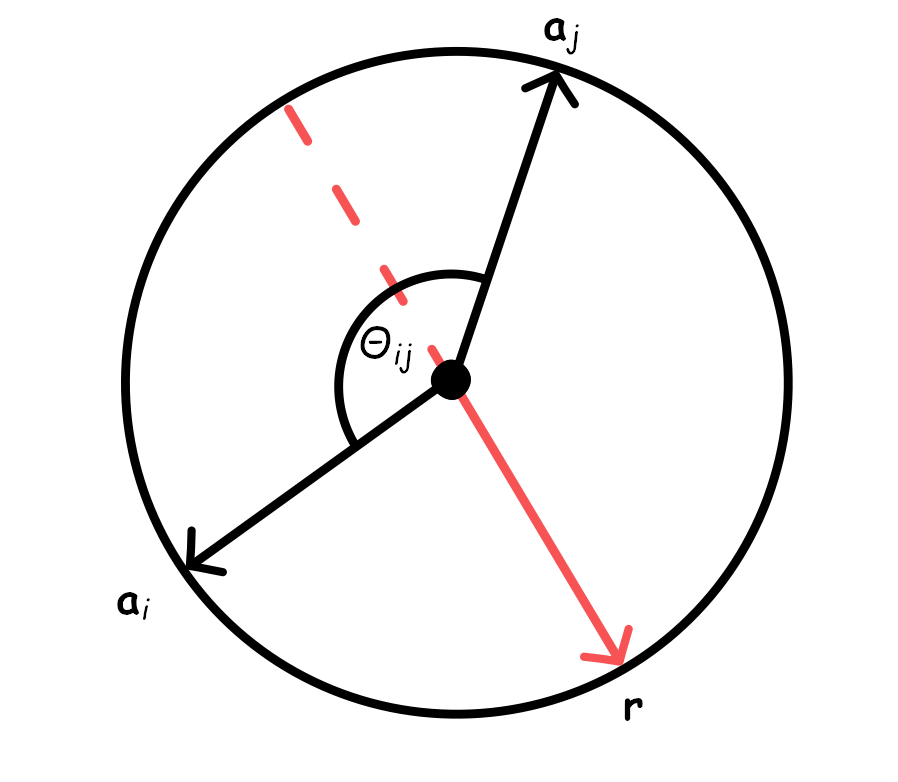
\includegraphics[width=0.5\textwidth]{img/lemma_plane.png}   
    \caption{Separace vrcholů $i$, $j$ náhodným vektorem $r$.}
    \label{fig:lemma_plane}
\end{figure}

\begin{lm}[KNUTH 2, 135]
    Nechť $x = (x_1, \dots, x_n)$ je vektor, jehož prvky jsou zvoleny nezávisle z normálního normovaného rozdělení $\mathcal{N}(0,1)$. Potom $r = \frac{x}{\| x \|}$ je náhodný vektor, který leží na jednotkové sféře $S_{n-1}$.
    \label{lemma:random-vector-on-sphere}
\end{lm}

Lemma~\ref{lemma:random-vector-on-sphere} nám dává postup, kterým provedeme bod \textbf{2} v algoritmu~\ref{alg:max-cut}. Nyní ukážeme, jak \uv{dobrou} aproximaci algoritmem~\ref{alg:max-cut} dostaneme. Označme
$$
    \alpha = \min_{0 \leq \Theta \leq \pi} \frac{2 \Theta}{\pi (1 - \cos \Theta)}.
$$
Snadno se ukáže, použitím derivace, že $\alpha \approx 0.87856$.

\begin{lm}
    Nechť $Y$ je náhodná veličina, která označuje součet vah hran, které vedou z $S$ do $\bar{S}$, nalezeny algoritmem~\ref{alg:max-cut}. Potom
    $$
        E\left[ Y \right] \geq \alpha \cdot RELAX.
    $$
\end{lm}

\begin{proof}
    Z definice čísla $\alpha$, pro $0 \leq \Theta \leq \pi$, dostáváme
    \begin{equation}
        \frac{\Theta}{\pi} = \frac{2 \Theta}{\pi (1 - \cos \Theta)} \cdot \frac{1 - \cos \Theta}{2} \geq \frac{\alpha}{2} (1 - \cos \Theta).
        \label{eq:proof_1}
    \end{equation}
    Použitím lemmatu~\ref{lemma:sep} a nerovnosti~\ref{eq:proof_1} dostáváme
    \begin{equation*}
        \begin{split}
            E\left[ Y \right] &= \sum w_{ij} P\left[ X_{ij} \right] \\
                              &= \sum w_{ij} \frac{\Theta_{ij}}{\pi} \\
                              &\geq \frac{\alpha}{2} \sum w_{ij} (1 - \cos \Theta_{ij}) \\
                              &= \alpha \cdot RELAX.
        \end{split}
    \end{equation*}
\end{proof}

\noindent Poznamenejme, že samozřejmě platí
\begin{equation}
    OPT \geq E\left[ Y \right] \geq \alpha \cdot RELAX.
    \label{eq:int-gap}
\end{equation}

\noindent \textbf{Mezeru celočíselnosti} relaxace (pro maximalizační problém) definujeme jako
$$
    \inf_{I} \frac{OPT(I)}{RELAX(I)},
$$
kde infimum probíhá přes všechny instance $I$ daného programu (pro minimalizační problém by se čitatel a jmenovat prohodily). Ze vztahu~\ref{eq:int-gap} dostáváme, že mezera celočíselnosti relaxace~\ref{eq:V-MAX-CUT} je alespoň $\alpha \approx 0.87856$.

Předchozí odvození je založeno na střední hodnotě náhodné veličiny $Y$. Proto kroky \textbf{2} a \textbf{3}, v algoritmu~\ref{alg:max-cut}, opakujeme vícekrát a jako výsledek zvolíme množinu $S$, která dává největší součet hran z $S$ do $\bar{S}$. Dále jen specifikujeme kolikrát musíme tyto kroky opakovat. Kompletní odvození je v \textbf{[REF]}. Zvolíme tedy $\varepsilon > 0$ (malé), nechť
$$
    c = \frac{\varepsilon \alpha}{2 + 2\varepsilon - \alpha},
$$
a kroky \textbf{2}, \textbf{3} opakujeme $\lceil \frac{1}{c} \rceil$-krát.


\section{Úloha MAX $k$-CUT}

V této části shrneme semidefinitní (vektorové) formulace s aproximačními schématy z několika článků pro úlohu MAX~$k$-CUT.

\subsection{Frieze-Jerrum a MAX $k$-CUT}

Začneme článkem \textbf{[REF]}. Uvažme rovnostranný simplex $\Sigma_k$ v $\mathbb{R}^{k-1}$ s vrcholy $b_1, b_2, \dots, b_k$. Nechť $c = (b_1 + \dots + b_k) / k$ je těžiště $\Sigma_k$ a nechť $a_i = b_i - c$, kde $i = 1, \dots, k$. Dále předpokládejme, že délka strany $\Sigma_k$ je taková, že $\| a_i\| = 1$.

\begin{lm}\textbf{[REF]}
    Pro $i \neq j$, platí
    $$
        \langle a_i, a_j \rangle = -\frac{1}{k-1}.
    $$
\end{lm}

\noindent Nyní můžeme formulovat úlohu MAX $k$-CUT následovně:

\begin{equation}\tag{FJ}
    \begin{split}
        &\max \frac{k-1}{k} \sum_{1 \leq i < j \leq n} w_{ij} (1 - \langle y_i, y_j \rangle) \\
        &y_i \in \left\{ a_1, \dots, a_k \right\}.
    \end{split}
    \label{eq:FJ}
\end{equation}

\noindent Poznamenejme, že
$$
    1 - \langle y_i, y_j \rangle = 
    \begin{cases}
        0           & y_i = y_j, \\
        k / (k - 1) & y_i \neq y_j.
    \end{cases}
$$

\noindent K získání vektorové relaxace programu~\ref{eq:FJ} nahradíme vektor $y_i$ vektorem $v_i$, kde $v_i$ je vektor na $S_{n-1}$.

\begin{equation}\tag{FJ-RELAX}
    \begin{split}
        &\max \frac{k}{k-1} \sum_{1 \leq i < j \leq n} w_{ij} (1 - \langle v_i, v_j \rangle) \\
        &\forall i \in V:\ \langle v_i, v_i \rangle = 1, \\
        &\forall i \neq j \in V:\ \langle v_i, v_j \rangle \geq -\frac{1}{k-1}, \\
        &\forall i \in V:\ v_i \in \mathbb{R}^n.
    \end{split}
    \label{eq:FJ-RELAX}
\end{equation}


Máme řešení $a_1, \dots, a_n$ programu~\ref{eq:FJ-RELAX}. Zvolíme $k$ náhodných vektorů $z_1, \dots, z_k$ na jednotkové sféře $S_{n-1}$. Pro každý vrchol $i \in V$ určíme $k$ skalárních součinů $\langle a_i, z_1 \rangle, \dots, \langle a_i, z_k \rangle$ a vrchol $i$ přidáme do množiny $V_j$, jestliže $j = \arg \max \left\{ \langle a_i, z_l \rangle \mid l = 1, \dots, k \right\}$. Použitím tohoto postupu dostáváme následující algoritmus.

\begin{alg}[FJ MAX $k$-CUT]$ $
    \begin{enumerate}
        \item Najdi řešení $a_1, \dots, a_n$ programu~\ref{eq:FJ-RELAX}.
        \item Zvol náhodně $k$ vektorů $z_1, \dots, z_k$ na jednotkové sféře $S_{n-1}$.
        \item Pro každý vrchol $i \in V$ určit $k$ skalárních součinů $\langle a_i, z_1 \rangle, \dots, \langle a_i, z_k \rangle$.
        \item Vrchol $i$ přidej do množiny $V_j$, jestliže $j = \arg \max \left\{ \langle a_i, z_l \rangle \mid l = 1, \dots, k \right\}$.
    \end{enumerate}
    \label{alg:fj-max-k-cut}
\end{alg}


\subsection{Goemans-Williamson a MAX $3$-CUT}

Algoritmus vycházející z článku \textbf{[REF]} využívá komplexní semidefinitní programování, tj. každý prvek je reprezentován komplexním vektorem. Následující vektorový program je relaxací úlohy MAX $3$-CUT, viz \textbf{[REF]}. 

\begin{equation}\tag{GW-RELAX}
    \begin{split}
        &\max \frac{2}{3} \sum_{1 \leq i < j \leq n} w_{ij} (1 - \langle v_i^1, v_j^1 \rangle) \\
        &\forall i \in V\ \forall a,b \in \left\{ 1,2,3 \right\}, a \neq b:\ \langle v_i^a, v_i^b \rangle = -\frac{1}{2}, \\
        &\forall i,j \in V\ \forall a,b,c \in \left\{ 1,2,3 \right\}:\ \langle v_i^a, v_i^b \rangle = \langle v_i^{a+c}, v_i^{b+c} \rangle \\
        &\forall i,j \in V\ \forall a,b \in \left\{ 1,2,3 \right\}:\ \langle v_i^a, v_j^b \rangle \geq -\frac{1}{2} \\
        &\forall i \in V\ \forall a \in \left\{ 1,2,3 \right\}:\ \langle v_i^a, v_i^a \rangle = 1 \\
        &\forall i \in V\ \forall a \in \left\{ 1,2,3 \right\}:\ v_i^a \in \mathbb{R}^{3n}
    \end{split}
    \label{eq:GW-RELAX}
\end{equation}


Mějme $3n$ vektorů, které tvoří řešení \ref{eq:GW-RELAX}. Pro vrchol $i \in V$ leží vektory $v_i^1, v_i^2, v_i^3$ ve stejné rovině tak, že jsou otočeny o $\frac{2\pi}{3}$. Nejprve zvolíme vektor $g \in \mathbb{R}^{3n}$ takový, že každá složka je vybrána nezávisle z normálního normovaného rozdělení $\mathcal{N}(0,1)$. Pro každý vrchol $i \in V$ určíme projekci vektoru $g$ do příslušné roviny. Odtud dostaneme úhel $\theta_i \in \langle 0, 2\pi)$ pro každý vrchol. Náhodně zvolíme úhel $\psi \in \langle 0, \pi)$ a vrchol $i \in V$ přidáme do množiny $V_j$, jestliže
$$
    \theta_i \in \psi + \frac{j 2 \pi}{3}, j \in \left\{ 0, 1, 2 \right\},
$$
kde úhly počítáme modulo $2$. Dostáváme algoritmus pro MAX $3$-CUT.

\begin{alg}[GW MAX $3$-CUT]$ $
    \begin{enumerate}
        \item Najdi řešení $a_1^1, a_1^2, a_1^3, \dots, a_n^3$ programu~\ref{eq:GW-RELAX}.
        \item Zvol náhodně vektor $g \in \mathbb{R}^{3n}$ tak, že každá složka je vybrána nezávisle z normálního normovaného rozdělelní $\mathcal{N}(0,1)$.
        \item Pro každý vrchol $i \in V$ urči projekci vektoru $g$ do příslušné roviny a vypočítej úhel $\theta_i$, který svírá projekce $g$ a vektor $a_i^3$.
        \item Zvol libovolně úhel $\psi \in \langle 0, \pi)$.
        \item Vrchol $i$ přidej do množiny $V_j$, jestliže $\theta_i \in \psi + \frac{j 2 \pi}{3}, j \in \left\{ 0, 1, 2 \right\}$, kde úhly počítáme modulo $2$.
    \end{enumerate}
    \label{alg:gw-max-3-cut}
\end{alg}


\subsection{Newman a MAX $k$-CUT}

Cílem \textbf{[REF]} je rozšířit přístup, pomocí komplexního semidefinitního programování, z \textbf{[REF]} pro MAX $3$-CUT na libovolné $k \geq 3$. Využívá se formulace \ref{eq:FJ-RELAX}, jejíž vyřešením dostaneme vektory $a_1, \dots, a_n$. Pro každý vrchol $i \in V$ definujeme dva ortonormální vektory v $\mathbb{R}^{2n}$ tak, že
$$
    u_i = \left( a_i, 0 \right) \text{ a } u_i^\bot = \left( 0, a_i \right).
$$

\noindent Dále zvolíme náhodný vektor $g \in \mathbb{R}^{2n}$, kde každá složka je vybrána náhodně z normálního normovaného rozdělení $\mathcal{N}(0,1)$. Pro každý vrchol $i \in V$ určíme projekci vektoru $g$ na $2$-dimenzionální disk
$$
    \left\{ u_i(\theta) \mid \theta \in \langle 0, \pi ) \right\},
$$
kde $u_i(\theta) = u_i \cos \theta + u_i^\bot \sin \theta, \theta \in \langle 0, \pi)$ a určíme úhel mezi projekcí vektoru $g$ a vektorem $u_i$. Nakonec náhodně zvolíme úhel $\psi \in \langle 0, 2 \pi )$ a vrchol $i \in V$ přidáme do množiny $V_j$, jestliže
$$
    \theta_i \in \psi + \frac{j 2 \pi}{k}, j \in \left\{ 0, 1, \dots, k-1 \right\},
$$
kde úhly počítáme modulo $2\pi$.

\begin{alg}[N1 MAX $k$-CUT]$ $
    \begin{enumerate}
        \item Najdi řešení $a_1, \dots, a_n$ programu~\ref{eq:FJ-RELAX}.
        \item Pro každý vrchol $i \in V$ urči vektory $u_i = (a_i, 0)$ a $u_i^\bot = (0, a_i)$ v $\mathbb{R}^{2n}$.
        \item Zvol náhodně vektor $g \in \mathbb{R}^{2n}$ tak, že každá složka je vybrána nezávisle z normálního normovaného rozdělení $\mathcal{N}(0, 1)$.
        \item Pro každý vrchol $i \in V$ urči úhel $\theta_i$.
        \item Zvol libovolně úhel $\psi \in \langle 0, 2 \pi )$ a vrchol $i \in V$ přidej do množiny $V_j$, jestliže $\theta_i \in \psi + \frac{j 2 \pi}{k}, j \in \left\{ 0, 1, \dots, k-1 \right\}$, kde úhly počítáme modulo $2\pi$.
    \end{enumerate}
    \label{alg:n-max-k-cut-1}
\end{alg}

V závěru článku je navrhnuté ještě jedno aproximační schéma. Shrneme ho v následujícím algoritmu.

\begin{alg}[N2 MAX $k$-CUT]$ $
    \begin{enumerate}
        \item Najdi řešení $a_1, \dots, a_n$ programu~\ref{eq:FJ-RELAX}.
        \item Zvol náhodně $k-1$ vektorů $g_1, \dots, g_{k-1} \in \mathbb{R}^n$ tak, že každá složka je vybrána nezávisle z normálního normovaného rozdělení $\mathcal{N}(0, 1)$.
        \item Vygeneruj rovnostranný simplex $\Sigma_k$ se středem v počátku.
        \item Pro každý vrchol $i \in V$ urči vektor $s_i = \left( \langle g_1, a_i \rangle, \dots, \langle g_{k-1}, a_i \rangle \right) \in \mathbb{R}^{k-1}$.
        \item Každý vektor (a tedy i vrchol) přiřaď k nejbližšímu vrcholu simplexu $\Sigma_k$.
    \end{enumerate}
    \label{alg:n-max-k-cut-2}
\end{alg}


\subsection{de Klerk-Pasechnik-Warners a MAX $k$-CUT}

Jako poslední ještě zmíníme algoritmus z \textbf{[REF]}, ve kterém nejprve vyřešíme následující semidefinitní program pro $\vartheta(\bar{G})$.

\begin{equation}\tag{THETA-$\bar{G}$}
    \begin{split}
        &\min t \\
        &\forall ij \in E:\ U_{ij} = -\frac{1}{t - 1} \\
        &\forall i \in V:\ U_{ii} = 1 \\
        &U \succeq 0, k \geq 2.
    \end{split}
    \label{eq:THETA-BAR-G}
\end{equation}

\noindent Dostaneme optimální řešení $(U, \vartheta(\bar{G}))$, kde matici $U$ použijeme k určení matice $Y$.
$$
    Y = U \otimes \frac{k}{k - 1} \left( I_k - \frac{1}{k} e_k e_k^T \right).
$$

\noindent Rozkladem $Y = V^TV$ získáme matici $V = \left[ v_1^1\ v_1^2\ \dots\ v_1^k\ \dots\ v_n^k \right]$.
Zvolíme náhodný vektor $g \in \mathbb{R}^{kn}$ na sféře $S_{kn-1}$ a určíme vektor $x$ tak, že
$$
    x_i^p = 
    \begin{cases}
        1  & g^T v_i^p = \max \left\{ \langle g, v_i^q \rangle \mid q = 1, \dots, k \right\}, \\
        -1 & \text{jinak.}
    \end{cases}
$$
Vektor $i \in V$ jsme přiřadili do množiny $V_j$, jestliže $x_i^j = 1$.


\section{Úloha CMAX $k$-CUT}

O obecné úloze CMAX $k$-CUT toho není mnoho známo. V \textbf{[REF]} (a později v jeho opravě \textbf{[REF]}) je popsán algoritmus, který využívá lokální prohledávání, jehož aproximační poměr je
$$
    \frac{t(k-1)}{2(s-1)+t(k-1)},
$$
kde $k\geq 2$, $t = \min_{i=1,\dots,k} |V_i|$ a $s = \max_{i=1,\dots,k} |V_i|$. Dále vyzkoušíme pro úlohu CMAX $k$-CUT přístup, ve kterém využijeme semidefinitní programování.

\subsection{Lokální prohledávání}

Nechť $G = (V,E)$ je neorientovaný graf s $n$ vrcholy. Označíme $w(u,v)$ váhu hrany $uv$. Na vstupu máme zadáno $k \geq 2$ a maximální počty vrcholů v jednotlivých množinách
$$
    |V_1| \leq s_1, \dots, |V_k| \leq s_k.
$$

Algoritmus začíná \textbf{inicializací}, kde libovolně rozdělíme vrcholy do $k$ množin tak, aby $|V_i| \leq s_i, i = 1, \dots, k$.

V \textbf{iteračním kroku} hledáme dvojici vrcholů $u \in V_i$ a $v \in V_j, i \neq j$, pro který
$$
    \sum_{x \in V_i, x \neq u} w(u,x) + \sum_{x \in V_j, x \neq v} w(v,x) > 
    \sum_{x \in V_j, x \neq u} w(u,x) + \sum_{x \in V_i, x \neq v} w(v,x) - 2 w(u,v).
$$
Pokud takové vrcholy najdeme, tak vrchol $u$ přesuneme do množiny $V_j$ a vrchol $v$ přesuneme do množiny $V_i$ a iterační krok opakujeme. Jestliže takové vrcholy neexistují algoritmus končí.

\subsection{CMAX $k$-CUT pomocí SDP}

V našem přístupu pro CMAX $k$-CUT použijeme algoritmus~\ref{alg:n-max-k-cut-2}, ze kterého potřebujeme rozklad vrcholů do množin $V_1, \dots, V_k$, vygenerovaný simplex a vektory příslušné jednotlivým vrcholům.

Máme zadány kapacity $s_1 \geq \dots \geq s_k$. Množiny, které dostaneme z algoritmu~\ref{alg:n-max-k-cut-2}, přeznačíme tak, aby součet záporných rezerv $r_i = s_i - |V_i|$ množin $V_1, \dots, V_k$ byl maximální.

Pro každou množinu $V_1, \dots, V_k$ určíme její rezervu $r_i$. Pokud jsou všechny rezervy nezáporné, vrátíme množiny $V_1, \dots, V_k$ jako výsledek. Jinak z množiny, která má zápornou rezervu vybereme vrchol, který má nejkratší vzdálenost do nějakého jiného vrcholu simplexu $\Sigma_k$. Takto iterujeme dokud nejsou všechny rezervy nezáporné.

\section{Experimenty}

K implementaci algoritmů je použit programovací jazyk Python 3 a framework Mosek. Jsou naimplementovány algoritmy~\ref{alg:fj-max-k-cut}, \ref{alg:gw-max-3-cut}, \ref{alg:n-max-k-cut-1}, \ref{alg:n-max-k-cut-2} pro úlohu MAX $k$-CUT a pro kapacitní verzi také algoritmus využívající lokální prohledávání a náš přístup využívající semidefinitní programování. Experimenty jsou realizovány na náhodných grafech řádu $30$ s předepsaným počtem hran. Tučně jsou vždy vyznačeny nejlepší výsledky.


\subsection{MAX $k$-CUT}

Pro úlohu MAX $3$-CUT byl otestován algoritmus~\ref{alg:fj-max-k-cut} a algoritmus~\ref{alg:gw-max-3-cut}.

\begin{table}[h!]
    \begin{center}
        \begin{tabular}{ c | c c | c c }
            $$ & \multicolumn{2}{c}{FJ MAX $k$-CUT} & \multicolumn{2}{c}{GW MAX $3$-CUT} \\
            $m$ & $100$ iterací & $10000$ iterací & $100$ iterací & $10000$ iterací \\
            \hline
            $43$  & $41$ & $\mathbf{43}$ & $37$ & $40$ \\
            $87$  & $80$ & $\mathbf{82}$ & $72$ & $77$ \\
            $130$ & $116$ & $\mathbf{117}$ & $104$ & $115$ \\
            $174$ & $150$ & $\mathbf{153}$ & $140$ & $147$ \\
            $217$ & $178$ & $\mathbf{182}$ & $166$ & $175$ \\
            $261$ & $208$ & $\mathbf{210}$ & $194$ & $203$ \\
            $304$ & $239$ & $\mathbf{241}$ & $226$ & $240$ \\
            $348$ & $263$ & $\mathbf{265}$ & $251$ & $261$ \\
            $391$ & $287$ & $\mathbf{289}$ & $281$ & $287$ \\
        \end{tabular}
    \end{center}
    \caption{MAX $3$-CUT na náhodných grafech řádu $30$.}
    \label{tab:max-3-cut-random}
\end{table}

Pro úlohy MAX $4$-CUT a MAX $5$-CUT byl otestován algoritmus~\ref{alg:fj-max-k-cut}, algoritmus~\ref{alg:n-max-k-cut-1} a algoritmus~\ref{alg:n-max-k-cut-2}.

\begin{table}[h!]
    \begin{center}
        \begin{tabular}{ c | c c | c c | c c }
            $$ & \multicolumn{2}{c}{FJ MAX $k$-CUT} & \multicolumn{2}{c}{N1 MAX $k$-CUT} & \multicolumn{2}{c}{N2 MAX $k$-CUT} \\
            $m$ & $100$ iterací & $10000$ iterací & $100$ iterací & $10000$ iterací & $100$ iterací & $10000$ iterací \\
            \hline
            $43$  & $\mathbf{43}$ & $\mathbf{43}$ & $39$ & $42$ & $42$ & $\mathbf{43}$ \\
            $87$  & $84$ & $\mathbf{87}$ & $76$ & $81$ & $85$ & $\mathbf{87}$ \\
            $130$ & $125$ & $\mathbf{129}$ & $114$ & $119$ & $127$ & $\mathbf{129}$ \\
            $174$ & $163$ & $\mathbf{164}$ & $149$ & $157$ & $161$ & $\mathbf{164}$ \\
            $217$ & $195$ & $201$ & $185$ & $188$ & $197$ & $\mathbf{202}$ \\
            $261$ & $229$ & $\mathbf{233}$ & $215$ & $225$ & $230$ & $\mathbf{233}$ \\
            $304$ & $265$ & $267$ & $249$ & $258$ & $263$ & $\mathbf{268}$ \\
            $348$ & $289$ & $\mathbf{294}$ & $277$ & $287$ & $292$ & $\mathbf{294}$ \\
            $391$ & $321$ & $\mathbf{323}$ & $312$ & $319$ & $319$ & $\mathbf{323}$ \\
        \end{tabular}
    \end{center}
    \caption{MAX $4$-CUT na náhodných grafech řádu $30$.}
    \label{tab:max-4-cut-random}
\end{table}

\begin{table}[h!]
    \begin{center}
        \begin{tabular}{ c | c c | c c | c c }
            $$ & \multicolumn{2}{c}{FJ MAX $k$-CUT} & \multicolumn{2}{c}{N1 MAX $k$-CUT} & \multicolumn{2}{c}{N2 MAX $k$-CUT} \\
            $m$ & $100$ iterací & $10000$ iterací & $100$ iterací & $10000$ iterací & $100$ iterací & $10000$ iterací \\
            \hline
            $43$  & $\mathbf{43}$ & $\mathbf{43}$ & $40$ & $\mathbf{43}$ & $\mathbf{43}$ & $\mathbf{43}$ \\
            $87$  & $\mathbf{87}$ & $\mathbf{87}$ & $78$ & $84$ & $\mathbf{87}$ & $\mathbf{87}$ \\
            $130$ & $128$ & $\mathbf{130}$ & $119$ & $123$ & $128$ & $\mathbf{130}$ \\
            $174$ & $167$ & $\mathbf{170}$ & $156$ & $160$ & $167$ & $\mathbf{170}$ \\
            $217$ & $206$ & $208$ & $194$ & $199$ & $204$ & $\mathbf{209}$ \\
            $261$ & $242$ & $\mathbf{244}$ & $229$ & $234$ & $\mathbf{244}$ & $243$ \\
            $304$ & $276$ & $\mathbf{282}$ & $263$ & $270$ & $279$ & $\mathbf{282}$ \\
            $348$ & $309$ & $311$ & $294$ & $302$ & $307$ & $\mathbf{312}$ \\
            $391$ & $337$ & $\mathbf{343}$ & $328$ & $336$ & $339$ & $342$ \\
        \end{tabular}
    \end{center}
    \caption{MAX $5$-CUT na náhodných grafech řádu $30$.}
    \label{tab:max-5-cut-random}
\end{table}


\subsection{CMAX $k$-CUT}

Pro úlohu CMAX $k$-CUT jsou porovnány dva algoritmy. Jeden využívající lokální prohledávání a druhý přístup, který je založen na semidefinitním programování.
